
\begin{figure}
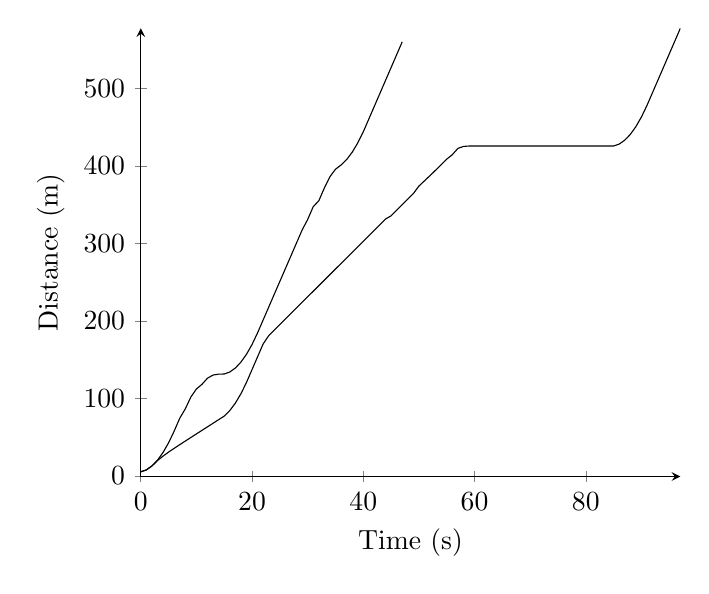
\begin{tikzpicture}
\begin{axis}[
legend style={anchor=west},
axis x line=bottom,
axis y line=left,
ymin=-1,
xlabel=Time (s),
ylabel=Distance (m),
]
\addplot[] coordinates {
(0, 5.1)
(1, 7.6)
(2, 12.6)
(3, 20.1)
(4, 30.1)
(5, 42.6)
(6, 57.6)
(7, 74.2)
(8, 86.34)
(9, 101.632252112)
(10, 112.059454389)
(11, 118.089689106)
(12, 126.079818867)
(13, 130.071924431)
(14, 131.27865093)
(15, 131.398797075)
(16, 134.018943221)
(17, 139.139089367)
(18, 146.759235512)
(19, 156.879381658)
(20, 169.499527803)
(21, 184.619673949)
(22, 201.219673949)
(23, 217.819673949)
(24, 234.419673949)
(25, 251.019673949)
(26, 267.519673949)
(27, 284.119673949)
(28, 300.719673949)
(29, 317.319673949)
(30, 330.919673949)
(31, 347.519673949)
(32, 355.049673949)
(33, 371.649673949)
(34, 386.170003201)
(35, 395.881144521)
(36, 401.296321513)
(37, 408.273383655)
(38, 417.750445797)
(39, 429.72750794)
(40, 444.204570082)
(41, 460.804570082)
(42, 477.404570082)
(43, 494.004570082)
(44, 510.604570082)
(45, 527.204570082)
(46, 543.804570082)
(47, 560.404570082)
};
\addplot[] coordinates {
(0, 5.1)
(1, 7.6)
(2, 12.6)
(3, 19.5616855662)
(4, 25.3799920277)
(5, 30.5631377019)
(6, 35.4295176435)
(7, 40.1485898144)
(8, 44.8017923926)
(9, 49.4262136994)
(10, 54.0383366955)
(11, 58.64543516)
(12, 63.2507467485)
(13, 67.8557672718)
(14, 72.4612629416)
(15, 77.0677237727)
(16, 84.1741846038)
(17, 93.780645435)
(18, 105.887106266)
(19, 120.493567097)
(20, 137.093567097)
(21, 153.693567097)
(22, 170.293567097)
(23, 180.893567097)
(24, 188.069089933)
(25, 195.244624587)
(26, 202.420172189)
(27, 209.595734014)
(28, 216.771311511)
(29, 223.946906334)
(30, 231.122520376)
(31, 238.298155819)
(32, 245.473815187)
(33, 252.649501417)
(34, 259.825217947)
(35, 267.00096883)
(36, 274.076758873)
(37, 281.259145184)
(38, 288.441532154)
(39, 295.62391989)
(40, 302.806308524)
(41, 309.988698219)
(42, 317.171089182)
(43, 324.353481677)
(44, 331.535876046)
(45, 335.718272742)
(46, 342.900901399)
(47, 350.083533345)
(48, 357.266169628)
(49, 364.448811797)
(50, 374.131453966)
(51, 380.897669891)
(52, 387.667240853)
(53, 394.634356394)
(54, 401.782183924)
(55, 408.930069052)
(56, 414.595366792)
(57, 422.760664533)
(58, 425.315898347)
(59, 425.837341426)
(60, 425.859957377)
(61, 425.859957377)
(62, 425.859957377)
(63, 425.859957377)
(64, 425.859957377)
(65, 425.859957377)
(66, 425.859957377)
(67, 425.859957377)
(68, 425.859957377)
(69, 425.859957377)
(70, 425.859957377)
(71, 425.859957377)
(72, 425.859957377)
(73, 425.859957377)
(74, 425.859957377)
(75, 425.859957377)
(76, 425.859957377)
(77, 425.859957377)
(78, 425.859957377)
(79, 425.859957377)
(80, 425.859957377)
(81, 425.859957377)
(82, 425.859957377)
(83, 425.859957377)
(84, 425.859957377)
(85, 425.859957377)
(86, 428.359957377)
(87, 433.359957377)
(88, 440.859957377)
(89, 450.859957377)
(90, 463.359957377)
(91, 478.359957377)
(92, 494.959957377)
(93, 511.559957377)
(94, 528.159957377)
(95, 544.759957377)
(96, 561.359957377)
(97, 577.959957377)
};

\end{axis}
\end{tikzpicture}
\label{tik:distance:100:18}
\caption{100 percent diving with GSC on route $18$}
\end{figure}
